\documentclass{beamer}
\usepackage{pgfpages}
\usepackage{newtxtext,newtxmath} %time new roman
%\setbeameroption{show notes}
%\setbeameroption{show notes on second screen=right}
\usetheme{Warsaw}
\usepackage[french]{babel}
\usepackage{csquotes}
\usepackage{tikz}
\pgfdeclareimage[width=0.5cm,height=0.5cm]{le-logo}{}
%\setbeamertemplate{footline}[frame number]
%Set number slide 

\usepackage[backend=biber]{biblatex}
%\usepackage[backend=biber, style=chem-acs]{biblatex}
\setbeamertemplate{bibliography item}[triangle]

\usepackage{multirow}% row fusion
\usepackage{array} % column fusion
\usepackage{xfrac} % small fractions
\usepackage{adjustbox}
\usepackage{listings}
\usepackage{color}
\definecolor{gray}{rgb}{0.4,0.4,0.4}
\definecolor{darkblue}{rgb}{0.0,0.0,0.6}
\definecolor{cyan}{rgb}{0.0,0.6,0.6}
 \titlegraphic{\vspace{-1cm}
      
\includegraphics[width=2.5cm]{images/logo_paris_8.png}\hspace*{4.75cm}~%
      \hfill
      
\includegraphics[width=2.5cm]{images/tc_logo.jpeg}
}
\setbeamertemplate{frametitle}{\nointerlineskip  
    \begin{beamercolorbox}[wd=\paperwidth,ht=2.75ex,dp=1.375ex]{frametitle}
        \hspace*{2ex}\insertframetitle \hfill {\small\insertframenumber/\inserttotalframenumber} \hspace*{1ex}%
    \end{beamercolorbox}}

\usecolortheme{wolverine}
\setbeameroption{hide notes} % Only slides


%%%%%%%%%%%%%%%%%%%%%%%%%%%
\title[Affectation de transaction à un store grace au Scoring] 
{Affectation de transaction à un store grace au Scoring}
%\subtitle {ne compléter que si l'article possède un sous-titre}
\author[Komlan Dantodji] 
{Komlan Jean-Marie DANTODJI}

\institute[]
{
  Etudiant en M1 Big Data, Université Paris 8
  \and
  Encadrante universitaire: Mme Rakia JAZIRI\\
  Encadrant entreprise:    Mr Thomas Moulin}
\date{Jun 17, 2020}


\begin{document}

\begin{frame}
  \titlepage
\end{frame}

\begin{frame}{Plan}
  \tableofcontents
\end{frame}

\section{Introduction}
\subsection{Présentation de l'entreprise}
\begin{frame}{Transaction Connect}
\begin{itemize}
		\item Start Up de B2B2C aux retailers
		\item Editeur de solution numerique basé sur la donnée de paiement
\end{itemize}
\end{frame}

\subsection{Solutions proposées}
\begin{frame}{Solutions proposées}
\begin{itemize}
		\item Transaction Connect signe des contrats avec des foncières
		\item Fournit des services et outils de décisions aux clients foncières (Dashboard, enrichissement des données)
		\item Fidélisation de la carte bancaire
		\item Notification et Validation des Cashbacks aux clients acheteurs
\end{itemize}
\end{frame}
\begin{frame}{Les modes d'intégrations des Clients Business (B)}
\begin{figure}[H]
    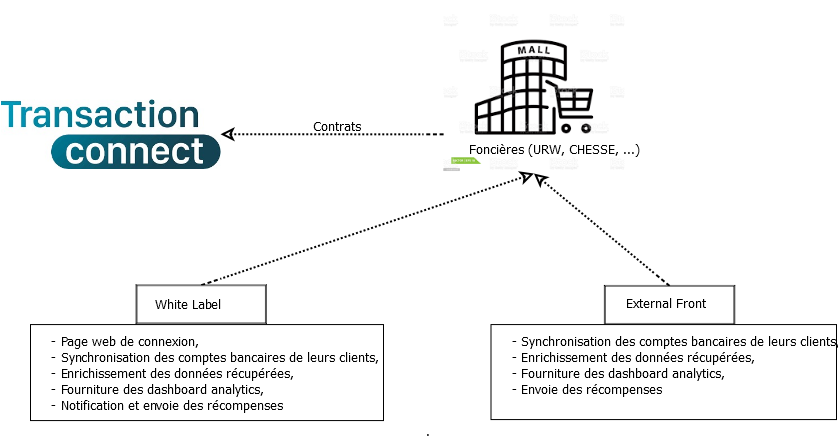
\includegraphics[width=11cm,height=4.8cm]{images/business_links.png}
    \caption{ modes d'intégration B}
    \label{fig:L1}
\end{figure}
\end{frame}
\begin{frame}{Les modes d'intégration des Clients C}
\begin{figure}[H]
    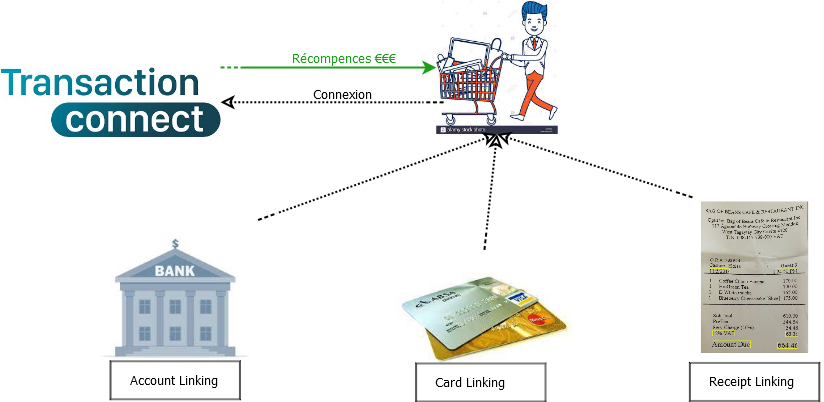
\includegraphics[width=11cm,height=4.8cm]{images/client_links.png}
    \caption{ Mode d'intégration C}
    \label{fig:L1}
\end{figure}
\end{frame}

\section{Problématique}
\begin{frame}{Problématique}
\begin{itemize}
		\item Les labels de transactions ne contiennent pas des informations nécessaires à l'affectation à un store
		\item Affectation des transactions à un store grace au scoring
		\item Automatisation des Modèles du scoring à un apprentissage mensuel
\end{itemize}
\end{frame} 

\section{Etat de l'art}
\subsection{Pattern Regex}
\begin{frame}{Etat de l'art: Pattern Regex}
\begin{itemize}
		\item Patterns Regex \\
				Exemple Label: "CB MONOPRIX 0295 Paris 02/03/21 10€" \\
				Retailer pattern: '.*\textbackslash mMONOPRIX\textbackslash M.*'\\
				Store pattern: '.*\textbackslash mMONOPRIX 0295\textbackslash M.*'
		\item Une transaction ayant ce label est affectable parcequ'on peut identifier le retailer MONOPRIX et le store MONOPRIX 0295
\end{itemize}
\end{frame} 
\subsection{Store Locator}
\begin{frame}{Etat de l'art: Store Locator}
\begin{itemize}
		\item Store Locator \\
				Exemple Label: "CB MONOPRIX Paris 02/03/21 10€" \\
				Ville: Paris\\
				Retailer pattern: '.*\textbackslash mMONOPRIX\textbackslash M.*'\\
		\item Si pour une transaction on connait la ville et le Retailer, Store Locator peut affecter cette transaction à un store si cette dernière est unique dans la ville
\end{itemize}
\end{frame} 
\subsection{Alpha / Alpha City}
\begin{frame}{Etat de l'art: Alpha / Alpha City}
\begin{itemize}
		\item Alpha / Alpha City (basé sur la détermination du Google Place Id d'une zone géographique)
\end{itemize}
\end{frame} 

\section{Algorithme du Scoring}
\begin{frame}{Algorithme du Scoring: Préalables}
\begin{itemize}
		\item Migration des requetes de calcule de Postgres vers Redshift Amazon
		\item Calcul des features nécessaires à l'apprentissage
\end{itemize}
\end{frame}
\begin{frame}{Features Engineering }
\begin{figure}[H]
    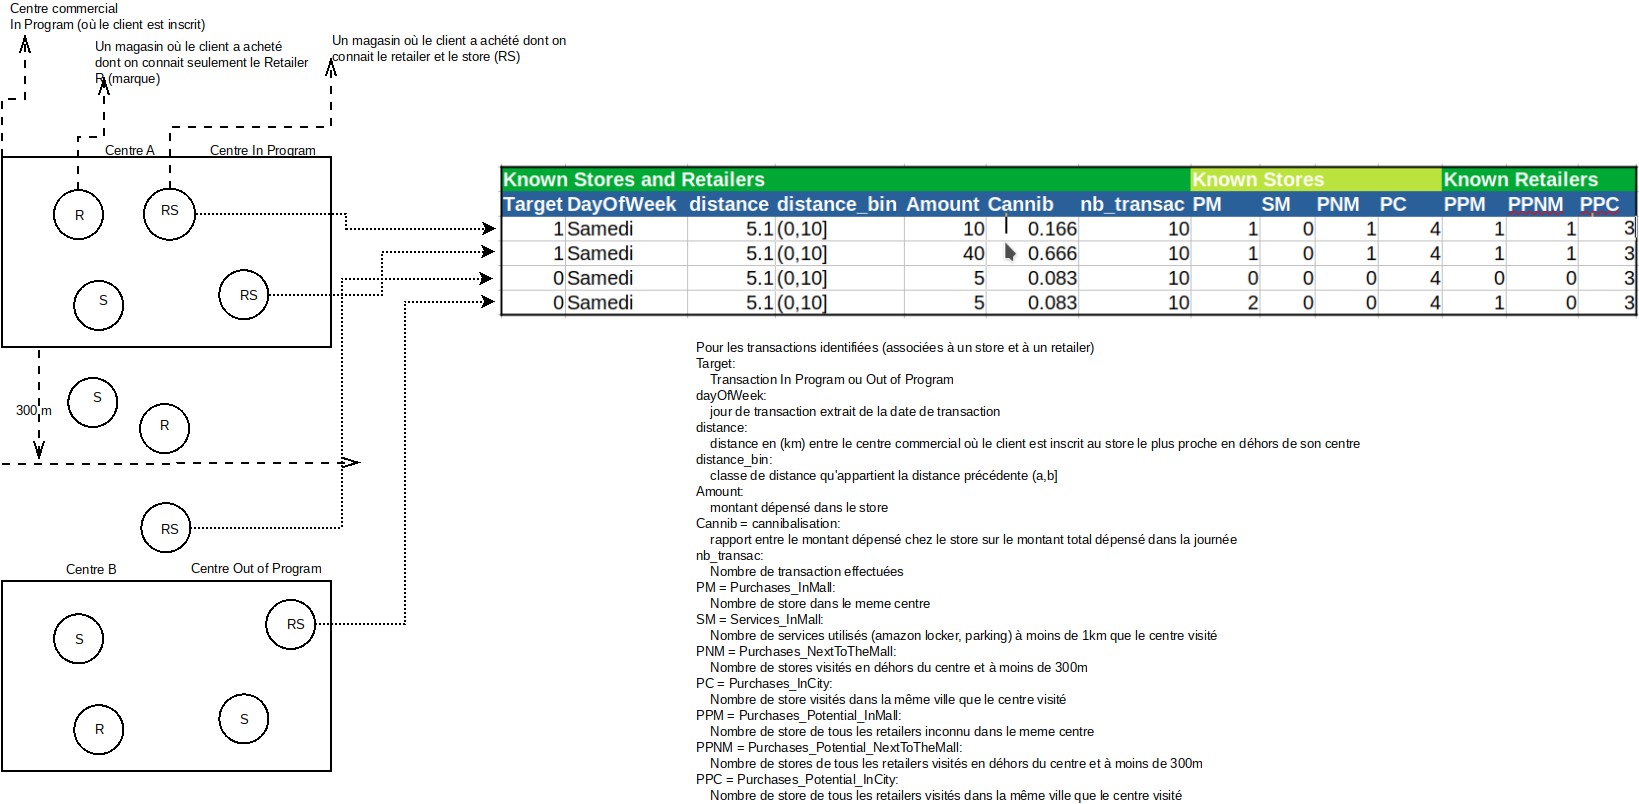
\includegraphics[width=11.5cm,height=5.5cm]{images/feature_engineering.png}
    \label{fig:L1}
\end{figure}
\end{frame}
\begin{frame}{Jeu de données}
\begin{itemize}
		\item Exemple de transactions du centre "Les 4 Temps" de Puteaux
\end{itemize}
\begin{figure}[H]
    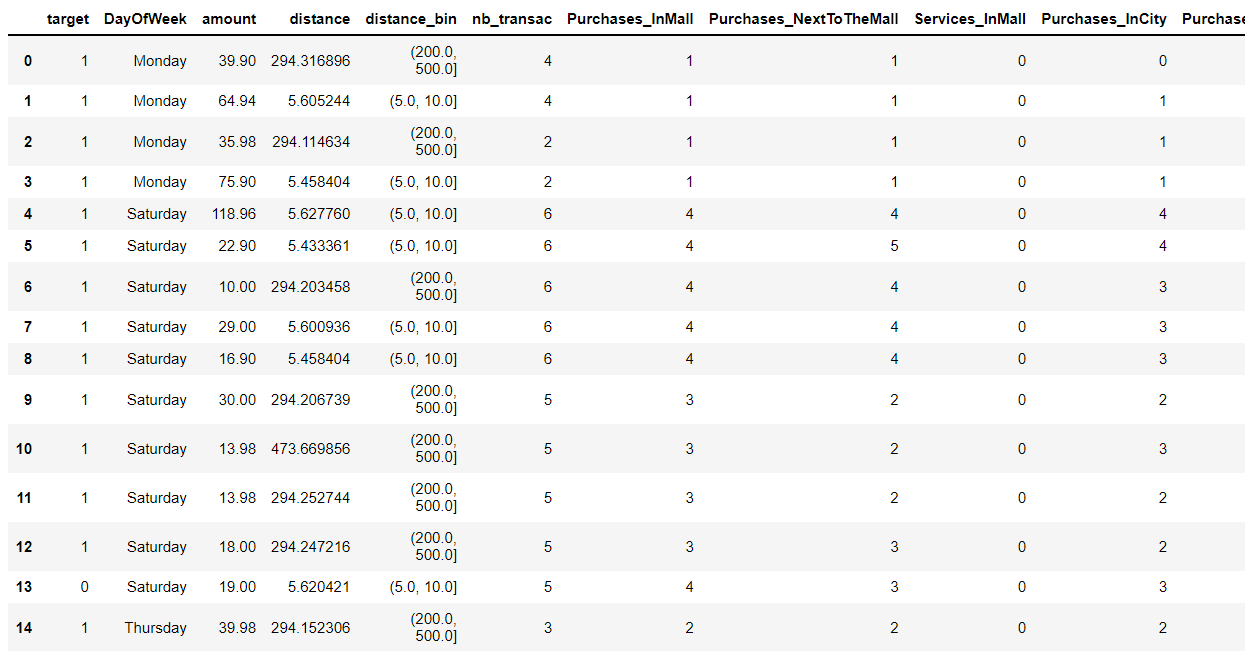
\includegraphics[width=12cm,height=4.5cm]{images/dataset_1.png}
    \caption{ Transactions considérées}
    \label{fig:L1}
\end{figure}
\end{frame}
\begin{frame}{Jeu de données}
\begin{figure}[H]
    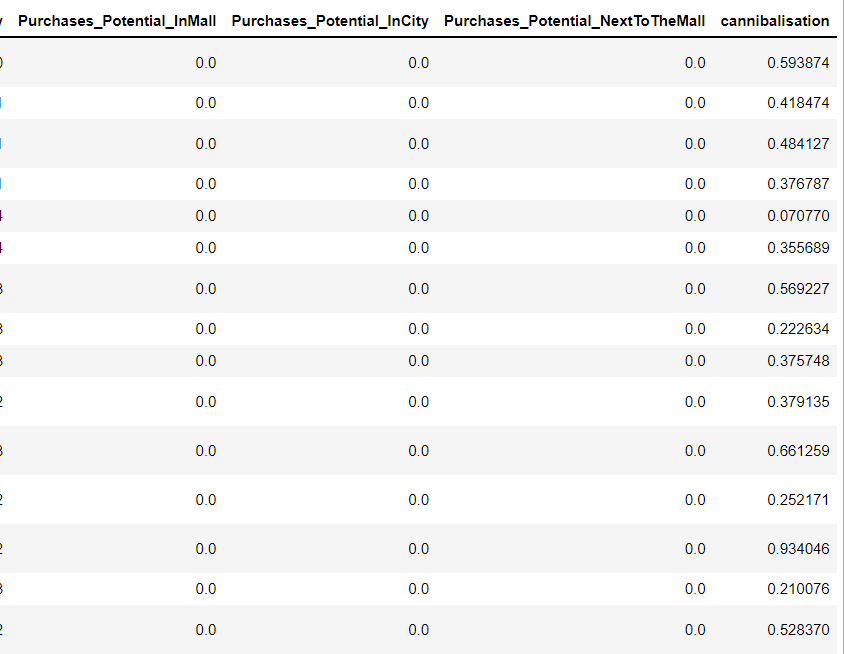
\includegraphics[width=11cm,height=5.1cm]{images/dataset_2.png}
    \caption{ Transactions considérées}
    \label{fig:L1}
\end{figure}
\end{frame} 
\begin{frame}{Informations données}
\begin{figure}[H]
    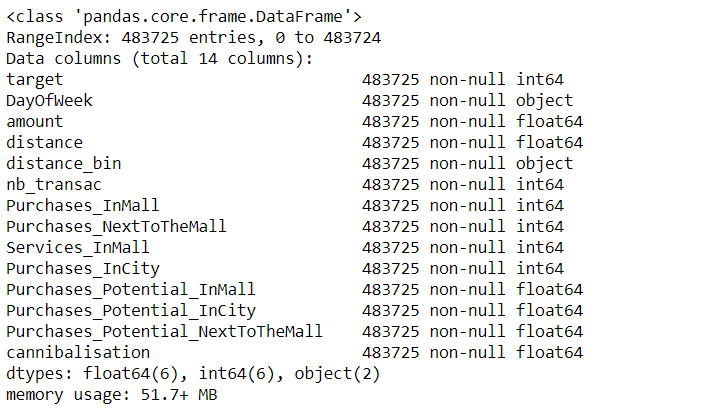
\includegraphics[width=11cm,height=5.1cm]{images/data_infos.png}
    \caption{ Les types de features}
    \label{fig:L1}
\end{figure}
\end{frame} 

\section{Apprentissage}
\begin{frame}{Apprentissage}
\begin{itemize}
		\item XGBoost
		\item Decision Tree
		\item Random Forest
\end{itemize}
\end{frame}




\section{Conclusion}
\begin{frame}{Conclusion}
\begin{itemize}
		\item Prochainement, Metrics de choix de modèle
		\item Ettendre le modele aux autres centres
		\item Créer un modele propre aux grands centres
		\item Automatiser l'apprentissage à chaque mois
\end{itemize}
\end{frame}


\begin{frame}
  \begin{block}{}
  \centering
  Merci pour votre attention...
  \end{block}
\end{frame}
\end{document}
